\documentclass[12pt,letterpaper]{article}
\usepackage{graphicx,textcomp}
\usepackage{natbib}
\usepackage{setspace}
\usepackage{fullpage}
\usepackage{color}
\usepackage[reqno]{amsmath}
\usepackage{amsthm}
\usepackage{fancyvrb}
\usepackage{amssymb,enumerate}
\usepackage[all]{xy}
\usepackage{endnotes}
\usepackage{lscape}
\newtheorem{com}{Comment}
\usepackage{float}
\usepackage{hyperref}
\newtheorem{lem} {Lemma}
\newtheorem{prop}{Proposition}
\newtheorem{thm}{Theorem}
\newtheorem{defn}{Definition}
\newtheorem{cor}{Corollary}
\newtheorem{obs}{Observation}
\usepackage[compact]{titlesec}
\usepackage{dcolumn}
\usepackage{tikz}
\usetikzlibrary{arrows}
\usepackage{multirow}
\usepackage{xcolor}
\newcolumntype{.}{D{.}{.}{-1}}
\newcolumntype{d}[1]{D{.}{.}{#1}}
\definecolor{light-gray}{gray}{0.65}
\usepackage{url}
\usepackage{listings}
\usepackage{color}

\definecolor{codegreen}{rgb}{0,0.6,0}
\definecolor{codegray}{rgb}{0.5,0.5,0.5}
\definecolor{codepurple}{rgb}{0.58,0,0.82}
\definecolor{backcolour}{rgb}{0.95,0.95,0.92}

\lstdefinestyle{mystyle}{
	backgroundcolor=\color{backcolour},  
	commentstyle=\color{codegreen},
	keywordstyle=\color{magenta},
	numberstyle=\tiny\color{codegray},
	stringstyle=\color{codepurple},
	basicstyle=\footnotesize,
	breakatwhitespace=false,        
	breaklines=true,                
	captionpos=b,                    
	keepspaces=true,                
	numbers=left,                    
	numbersep=5pt,                  
	showspaces=false,                
	showstringspaces=false,
	showtabs=false,                  
	tabsize=2
}
\lstset{style=mystyle}
\newcommand{\Sref}[1]{Section~\ref{#1}}
\newtheorem{hyp}{Hypothesis}

\title{Problem Set 2}
\date{Due: October 23, 2025}
\author{Applied Stats/Quant Methods 1/Nour Kebbi/ Answer Sheet}

\begin{document}
	\maketitle
	\section*{Instructions}
	\begin{itemize}
		\item Please show your work! You may lose points by simply writing in the answer. If the problem requires you to execute commands in \texttt{R}, please include the code you used to get your answers. Please also include the \texttt{.R} file that contains your code. If you are not sure if work needs to be shown for a particular problem, please ask.
		\item Your homework should be submitted electronically on GitHub.
		\item This problem set is due before 23:59 on Thursday October 23, 2025. No late assignments will be accepted.
		
	\end{itemize}
	
	
	\vspace{.5cm}
	\section*{Question 1: Political Science}
	\vspace{.25cm}
	The following table was created using the data from a study run in a major Latin American city.\footnote{Fried, Lagunes, and Venkataramani (2010). ``Corruption and Inequality at the Crossroad: A Multimethod Study of Bribery and Discrimination in Latin America. \textit{Latin American Research Review}. 45 (1): 76-97.} As part of the experimental treatment in the study, one employee of the research team was chosen to make illegal left turns across traffic to draw the attention of the police officers on shift. Two employee drivers were upper class, two were lower class drivers, and the identity of the driver was randomly assigned per encounter. The researchers were interested in whether officers were more or less likely to solicit a bribe from drivers depending on their class (officers use phrases like, ``We can solve this the easy way'' to draw a bribe). The table below shows the resulting data.
	
	\newpage
	\begin{table}[h!]
		\centering
		\begin{tabular}{l | c c c }
			& Not Stopped & Bribe requested & Stopped/given warning \\
			\\[-1.8ex]
			\hline \\[-1.8ex]
			Upper class & 14 & 6 & 7 \\
			Lower class & 7 & 7 & 1 \\
			\hline
		\end{tabular}
	\end{table}
	
	\begin{enumerate}
		
		\item [(a)]
		Calculate the $\chi^2$ test statistic by hand/manually (even better if you can do "by hand" in \texttt{R}).\\
		\vspace{0cm}
		
		\lstinputlisting[language=R, firstline=6, lastline=33]{PS02_NK.R}
		\vspace{1cm} The test statistic is 3.791168.
		\newpage
		\item [(b)]
		Now calculate the p-value from the test statistic you just created (in \texttt{R}).\footnote{Remember frequency should be $>$ 5 for all cells, but let's calculate the p-value here anyway.}  What do you conclude if $\alpha = 0.1$?\\
		\lstinputlisting[language=R, firstline=36, lastline=39]{PS02_NK.R}
		\vspace{.25cm} Since the p-value is 0.1502306 and alpha = 0.1 then p-value is greater than alpha and hence, we fail to reject the Null Hypothesis that the variables are statistically independent.\\
		
		\item [(c)] Calculate the standardized residuals for each cell and put them in the table below.
		\vspace{0.25cm}
		
		\begin{table}[h]
			\centering
			\begin{tabular}{l | c c c }
				& Not Stopped & Bribe requested & Stopped/given warning \\
				\\[-1.8ex]
				\hline \\[-1.8ex]
				Upper class  & 0.322 & -1.642 & 1.523 \\
				\\
				Lower class & -0.322 & 1.642  & -1.523  \\
				
			\end{tabular}
		\end{table}
		\lstinputlisting[language=R, firstline=44, lastline=68]{PS02_NK.R}
		\item [(d)] How might the standardized residuals help you interpret the results?  
		

		\vspace{.25cm} We can see from the standarized residuals that upper class drivers are mosre likely to be stopped given the residual is 1.523 than being asked for a bribe (-1.642) or than not being stopped (0.322). We can also see that lower class drivers are more likely to be asked for a bribe given the residual is 1.642 than being stopped (-1.523) or than not being stopped (-0.322).
	\end{enumerate}
	
	\section*{Question 2: Economics}
	Chattopadhyay and Duflo were interested in whether women promote different policies than men.\footnote{Chattopadhyay and Duflo. (2004). ``Women as Policy Makers: Evidence from a Randomized Policy Experiment in India. \textit{Econometrica}. 72 (5), 1409-1443.} Answering this question with observational data is pretty difficult due to potential confounding problems (e.g. the districts that choose female politicians are likely to systematically differ in other aspects too). Hence, they exploit a randomized policy experiment in India, where since the mid-1990s, $\frac{1}{3}$ of village council heads have been randomly reserved for women. A subset of the data from West Bengal can be found at the following link: \url{https://raw.githubusercontent.com/kosukeimai/qss/master/PREDICTION/women.csv}\\
	
	\noindent Each observation in the data set represents a village and there are two villages associated with one GP (i.e. a level of government is called "GP"). Figure~\ref{fig:women_desc} below shows the names and descriptions of the variables in the dataset. The authors hypothesize that female politicians are more likely to support policies female voters want. Researchers found that more women complain about the quality of drinking water than men. You need to estimate the effect of the reservation policy on the number of new or repaired drinking water facilities in the villages.
	\vspace{.5cm}
	\begin{figure}[h!]
		\caption{\footnotesize{Names and description of variables from Chattopadhyay and Duflo (2004).}}
		\vspace{.5cm}
		\centering
		\label{fig:women_desc}
		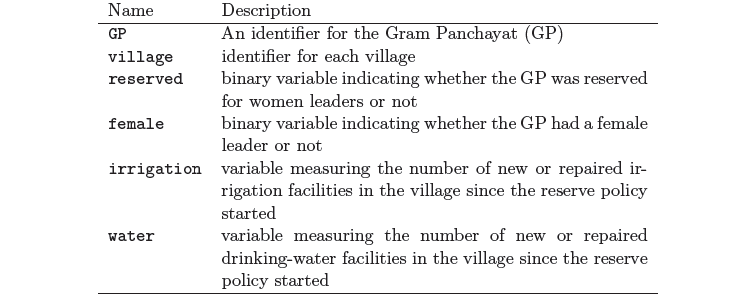
\includegraphics[width=1.1\textwidth]{women_desc.png}
	\end{figure}
	
	\newpage
	\begin{enumerate}
		\item [(a)] State a null and alternative hypothesis (two-tailed).
		\newline
		\vspace{.25cm} Ho null hypothesis: having a reservation policy (female) head has no effect on the number of new/repaired drinking water facilities in villages. The alternative hypothesis: having a reservation policy (no female) head has a positive or negative effect on the number of new/repaired drinking water facilities in villages.
		
		
		\vspace{0.5cm}
		\item [(b)] Run a bivariate regression to test this hypothesis in \texttt{R} (include your code!).
		\lstinputlisting[language=R, firstline=81, lastline=103]{PS02_NK.R}
		\vspace{1cm} Betais 9.252423 and Alpha is 14.73832
		\vspace{1cm}
		\item [(c)] Interpret the coefficient estimate for reservation policy.
		\newline
		\vspace{1cm}Beta is 9.252423 and alpha is 14.73832 and beta now is >0 so villages with female heads (reservation policy) have more drinking water, around +9.252423 than villages withoutfemale heads. On average, a female head reservation policy leads to a 9.252423 increase in drinking water. The Alpha is 14.73832, so villages without female heads have around 14.73832 new/repaired drinking water. When there is no reservation policy (no female heads), the predicted value of new / repaired drinking water is 14.73832. Note that is may not be a meaningful quantity.
	\end{enumerate}
	
	
	%\end{enumerate}
\end{document}